%
% File acl2016.tex
%
%% Based on the style files for ACL-2015, with some improvements
%%  taken from the NAACL-2016 style
%% Based on the style files for ACL-2014, which were, in turn,
%% Based on the style files for ACL-2013, which were, in turn,
%% Based on the style files for ACL-2012, which were, in turn,
%% based on the style files for ACL-2011, which were, in turn, 
%% based on the style files for ACL-2010, which were, in turn, 
%% based on the style files for ACL-IJCNLP-2009, which were, in turn,
%% based on the style files for EACL-2009 and IJCNLP-2008...

%% Based on the style files for EACL 2006 by 
%%e.agirre@ehu.es or Sergi.Balari@uab.es
%% and that of ACL 08 by Joakim Nivre and Noah Smith

\documentclass[12pt]{article}
\usepackage{acl2016}
\usepackage{times}
\usepackage{url}
\usepackage{latexsym}
\usepackage{graphicx}

\graphicspath{ {.} }

\aclfinalcopy % Uncomment this line for the final submission
%\def\aclpaperid{***} %  Enter the acl Paper ID here

%\setlength\titlebox{5cm}
% You can expand the titlebox if you need extra space
% to show all the authors. Please do not make the titlebox
% smaller than 5cm (the original size); we will check this
% in the camera-ready version and ask you to change it back.

\newcommand\BibTeX{B{\sc ib}\TeX}

\title{Assessing a Word Similarity Model for Determining Overall Category}

\author{Ethan Campbell-Taylor \\
Linguistics '16\\\And
  Becky Marvin \\
  Cognitive Science '16 \\
  \\\And
  Harvey Xia \\
  Computer Science '16 \\}

\date{May 9, 2016}

\begin{document}
\maketitle
\begin{abstract}
  This document contains the methodology and results of a study examining the effectiveness of using WordNet's semantic hierarchy information to classify text documents. We used the semantic similarity information from WordNet, in addition to a hierarchical clustering algorithm to determine the similarity of the nouns in a given text document. We then found the hypernyms of the resulting clusters and compared the hypernyms to the labeled categories of the document. We assessed the accuracy of our algorithm by comparing its judgments of overall categories to the actual labeled categories of documents.
\end{abstract}

\section{Introduction}

Text classification has previously been researched using ``bag of words'' representations of word meanings and a multitude of statistical methods such as generative models and discriminative models. We explore a different, non-statistical approach in this paper, that of using WordNet's available semantic similarity information combined with a hierarchical clustering algorithm to determine the overall category of a text document. We believe this approach has potential to be a promising model for representing the semantic information in a given document, which could be useful in determining the overall semantic category of a document.

\section{Motivation}

A document's semantic meaning is partially represented by the set of nouns that appear in the document. Our hypothesis is that the set of nouns of any given document are semantically related and that this semantic structure can be used to infer the document's semantic meaning as a whole, in particular its content category. Trivially, a document's content can be represented as its set of nouns. We wish to use WordNet's semantic hierarchy to synthesize the set of nouns into a reduced set of synsets, i.e. noun senses, that capture the overall category of the document in a more cohesive way. For instance, we would like our model to say that a document is about "canines" rather than about "dogs," "wolves", and "foxes." This synset synthesis is accomplished through using WordNet to find lowest common hypernyms for sets of synsets. Furthermore, we would like to return a set of synsets that are ranked according to their salience to the document's overall meaning.

\section{Our Model}\label{model}

\subsection{The Algorithm}

The following is a high level overview of our classification algorithm for a single document. Each step is annotated with the corresponding Python file in bold.

\begin{enumerate}  
\item Extract all nouns, \textbf{noun\_extractor.py}. For each line:
\begin{enumerate}
\item Strip all punctuation and non-ascii characters.
\item Tokenize the line.
\item Tag the POS of each token.
\item Filter out all non-noun tokens.
\item Add all noun tokens to a Python dictionary as keys whose values are the counts of the token.
\end{enumerate}
\item Use WordNet to look up synsets for each noun token. Remove nouns for which no synset exists, \textbf{cluster.py}.
\item Generate a 2-dimension matrix of similarity values for each pairwise combination of synsets. Similarity values are looked up using WordNet.
\item Perform hierarchical clustering on the synsets.
\item Select a particular subset of clusters based on min\_size, max\_size, and max\_dist parameters, \textbf{semantic\_classifier.py}.
\item Sort clusters by noun token occurrence, most frequent to least.
\item Find the lowest common hypernym (i.e. lowest common ancestor) for each cluster of synsets.
\end{enumerate}

\subsection{Description of Algorithm}

Since our model is attempting to determine the category of a document based on the nouns used in it, the first step in our algorithm is to extract all the document's nouns. After removing punctuation and non-ascii characters, the algorithm tokenizes each line and tags the tokens with nltk's part of speech tagger. 

It then stems the relevant nouns, determined by whether their stemmed versions exist in wordnet. We removed the stems of words ending in ``ing,'' ``s,'' ``e,'' ``able,'' ``y,'' and ``er.'' For example, ``photography'' becomes ``photograph,'' but ``agency'' remains as is, since ``agenc'' is not recognized as a word by WordNet. After stemming, the algorithm counts every instance of each token and stores this information in a Python dictionary. For each of these tokens, the algorithm finds the corresponding synset (the set of senses listed in WordNet for the word) if it exists. These synsets are used to compute similarity measures for the purposes of clustering.

Stemming is motivated by the observation that some semantically related nouns are considered as relatively dissimilar according to WordNet. For instance, WordNet ranks "photograph" and "painting" as more similar than "photograph" and "photography." Strictly speaking, there is a sense in which "painting" is more similar to "photograph" than "photography" is—a painting and a photograph are both flat objects that contain an image, whereas photography is a process of producing images. Therefore it makes sense that WordNet places "photograph" and "photography" in different sections of the semantic tree. For our purposes of determining a document's semantic subjects, however, this WordNet's distinction between "photograph" and "photography" are too fine-grained. Collapsing those two nouns into a single noun "photograph" improves our algorithm's performance as it improves the signal for "photograph" being a salient semantic category.

Having done this, the algorithm computes a similarity matrix for every pair of nouns in the document: that is, it calculates and stores the similarity of the synsets for each noun pair. We use Wu-Palmer similarity as a measure of how similar two synsets are. Wu-Palmer similarity for synsets $s1$ and $s2$, where $lcs$ is the least common hypernym, i.e. the more informative semantic class that encloses both $s1$ and $s2$, is given by:\\

$2*depth(lcs) / (depth(s1) + depth(s2))$\\

We used the fastcluster library to do heirarchical clustering. Then we choose clusters based on three parameters: the minimum size of the cluster, the maximum size of the cluster, and the maximum distance of the cluster (a cluster's distance is a measure of how far apart elements in the cluster are from each other, distance in this case being Wu-Palmer similarity between synsets). Figure 1 shows a visual representation of the result of hierarchical clustering on synsets where the X-axis consists of the constituent synsets and the Y-axis represents distance of clusters.

\begin{figure*}[t]
\caption{Dendrogram representation of hierarchical clustering on synsets}
\centering
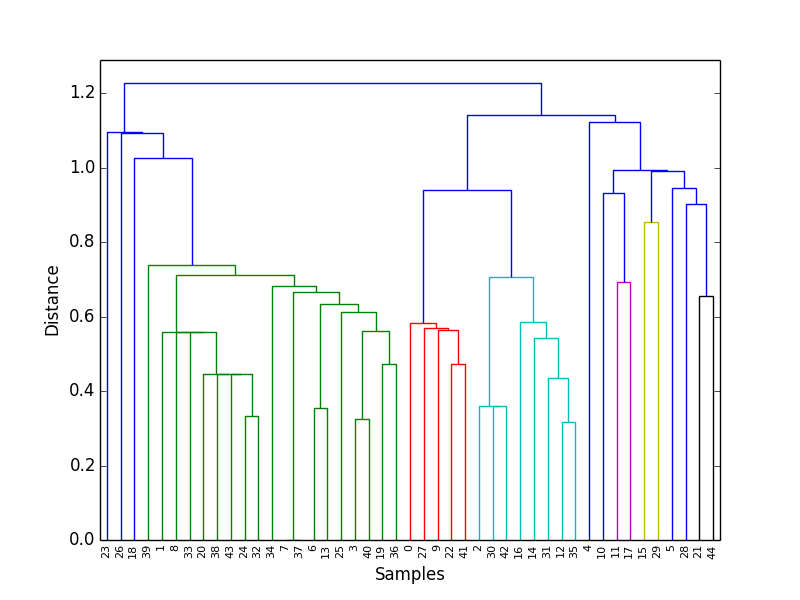
\includegraphics[width=\textwidth]{hca}
\end{figure*}

One interesting observation about choosing the set of clusters is that the larger the cluster size, the farther apart and thus more dissimilar its constituent synsets. Finding the lowest common hypernym of large clusters with large distances yields less informative hypernyms. In the extreme case, if the cluster contains a sufficiently diverse set of synsets, the lowest common hypernym becomes the root of the WordNet semantic tree, "entity." Larger cluster sizes, however, give the algorithm greater potential in synthesizing synsets into a particular hypernym. In the trivial case, the algorithm could simply return the set of nouns of the document as its representation of the document's semantic class. The ideal algorithm, however, would perform some degree of synthesis amongst the nouns and "infer" relevant semantic categories from constituent nouns. Because of this trade off between potential synthesis of nouns and a decrease in hypernym informativity, our algorithm exposes these parameters to the programmer to allow them to adjust the parameters according to their particular needs.

We chose to exclude clusters smaller than size 2 and larger than size 99, as well as those with a distance of less than 0.5. The clusters are then sorted by size, those with the greatest number of raw tokens appearing first. Finally, for each cluster, the algorithm finds the hypernym (the least common ancestor of all the synsets in the cluster).

The algorithm evaluates performance by finding the item in the hypernyms returned by our algorithm that is most similar to a tag for each labeled tag of the text document. We use Wu-Palmer similarity as a measure of how similar two words are according to WordNet.

\section{Evaluation}

We tested our algorithm on 295 articles taken from NPR's website, since these articles contained tags describing what the article was about. On average, the articles contained about 925 words, 135 of which were nouns. Of these 135 nouns, there were on average 87 distinct nouns. These nouns were then clustered by our algorithm and the hypernyms were created for each cluster. The most similar hypernym was computed for each tag for the article, and this similarity score (which took on values from 0 to 1) was then summed for all the tags and divided by the number of tags. That is, our overall similarity score for each document was:

\[
 \frac{1}{\#_{tags}} \sum_{t \in tags}{(\max_{h \in hypernyms}{wupSimilarity(h, t)})}
\]

This score would be closer to 1 if the closest hypernym for each tag was highly similar, and closer to 0 if the closest hypernym for each tag was highly dissimilar.

\section{Results}

We computed these similarity scores explained above for each article, and the resulting distribution of scores for each article is shown in Figure \ref{scoreHist}.

\begin{figure*}[h]
\centering
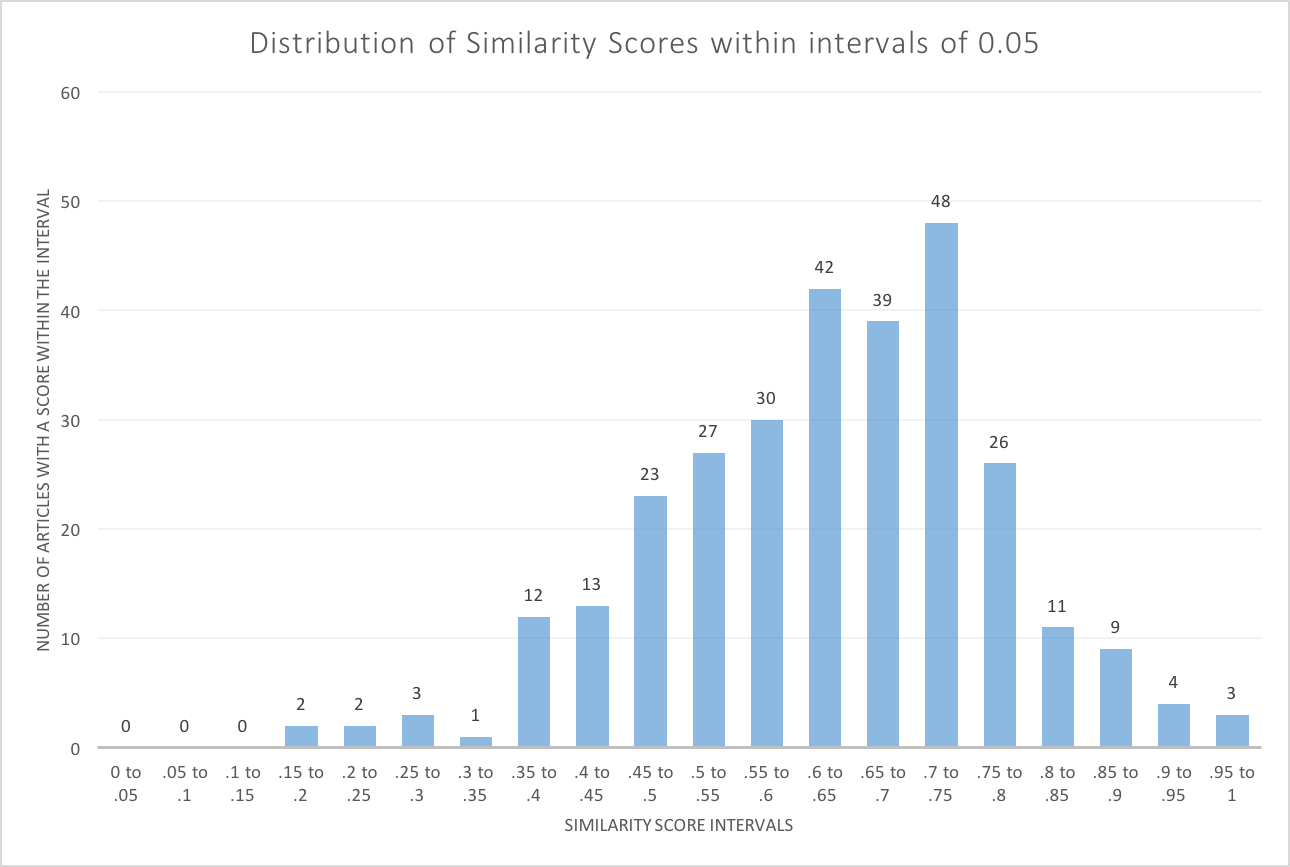
\includegraphics[width=\textwidth]{../scoreHist.png}
\caption{Distribution of scores.}
\label{scoreHist}
\end{figure*}

The distribution of scores roughly approximates a bell curve, with the center lying somewhere between 0.65 and 0.7. In fact, the average similarity score for all articles was 0.63. Notably, no articles had average similarity scores of less than 0.15, and three articles had similarity scores between 0.95 and 1.

Some tags were used for multiple articles, but there were 566 distinct tags used overall. Depending on the hypernyms produced by our algorithm for each article, these tags could be most similar to different hypernyms. For example, one article tagged as being about ``ebola'' was most similar to the hypernym ``joy,'' while a different article about ``ebola'' was most similar to the hypernym ``ill\_health.'' We computed the average number of different hypernyms matched with each distinct tag to determine whether our algorithm truly got a sense of what the article was about. On average, each tag was matched with 1.6 different hypernyms at the end of the algorithm.

\section{Issues and Further Work}

When looking up a synset for a particular noun token, WordNet returns a list of possible synsets if that noun token has multiple senses, sorted in order of most commonly appearing sense first. Our algorithm currently chooses the first synset i.e. the most common sense of the noun. But this is of course an approximation as the most common sense is not necessarily the correct sense used in the context of the document. This therefore introduces noise into our results. Selecting the correct sense of a noun token is a difficult problem that requires the algorithm to not only understand the context in which the noun token appears, but to be able to infer from the context what the most plausible sense is.

Another potential concern is that a considerable number of the nouns in the documents examined did not have WordNet entries. There are a few reasons for this: firstly, the majority of the articles we ran our algorithm on were health articles. As a result, many of the nouns used in the articles were medical in nature, and often did not have entries in WordNet. There are of course non-medical nouns that do not have entries, particularly proper nouns. In total, 1802 noun tokens did not have WordNet entries, which corresponds to an average of 5\% of the nouns in each document. As mentioned in Section \ref{model}, we had to remove nouns with no synsets before doing clustering. The exclusion of these nouns means the returned hypernyms are not as accurate as we would prefer. This is especially concerning considering that articles with a large number of nouns with very specific semantics (i.e. nouns less likely to have WordNet entries, such as medical nouns) are more likely to be about some topic in that semantic field. It is likely, then, that the omission of all these nouns has a significant detrimental effect on the hypernyms returned.

A similar issue is that some of the tags NPR uses on their articles do not have entries in WordNet. These tags may be proper nouns, multiple words, or words with specific semantics. As a result, we had to manually modify or remove these tags from the articles. Multiple-word tags were typically split into separate tags, leaving out function words such as ``the.'' Other tags were simply shortened; one of the most common tags was ``zika virus,'' which we changed to ``virus'' for articles that didn't already have a ``virus'' tag. Removing and modifying tags presumably affects the similarity scores between the hypernyms and the tags for the article, which confounds our ability to evaluate the model. A better method for future refinements of this algorithm might be to manually tag articles rather than using those included in the source.

\section{Discussion}



% include your own bib file like this:
%\bibliographystyle{acl}
%\bibliography{acl2016}
\bibliography{acl2016}
\bibliographystyle{acl2016}

\end{document}
